\section{Self-Organizing Maps (SOM)}

\mode<presentation>{
\begin{frame} 
    \begin{center} \huge
        \secname
    \end{center}
    \begin{center}
		Neighborhood-preserving clustering to explain the data
    \end{center}
\end{frame}
}

\subsection{The model class}

\begin{frame}{\subsecname:~The components SOM model}

\only<1-2>{
\svspace{-3mm}
\begin{center}
	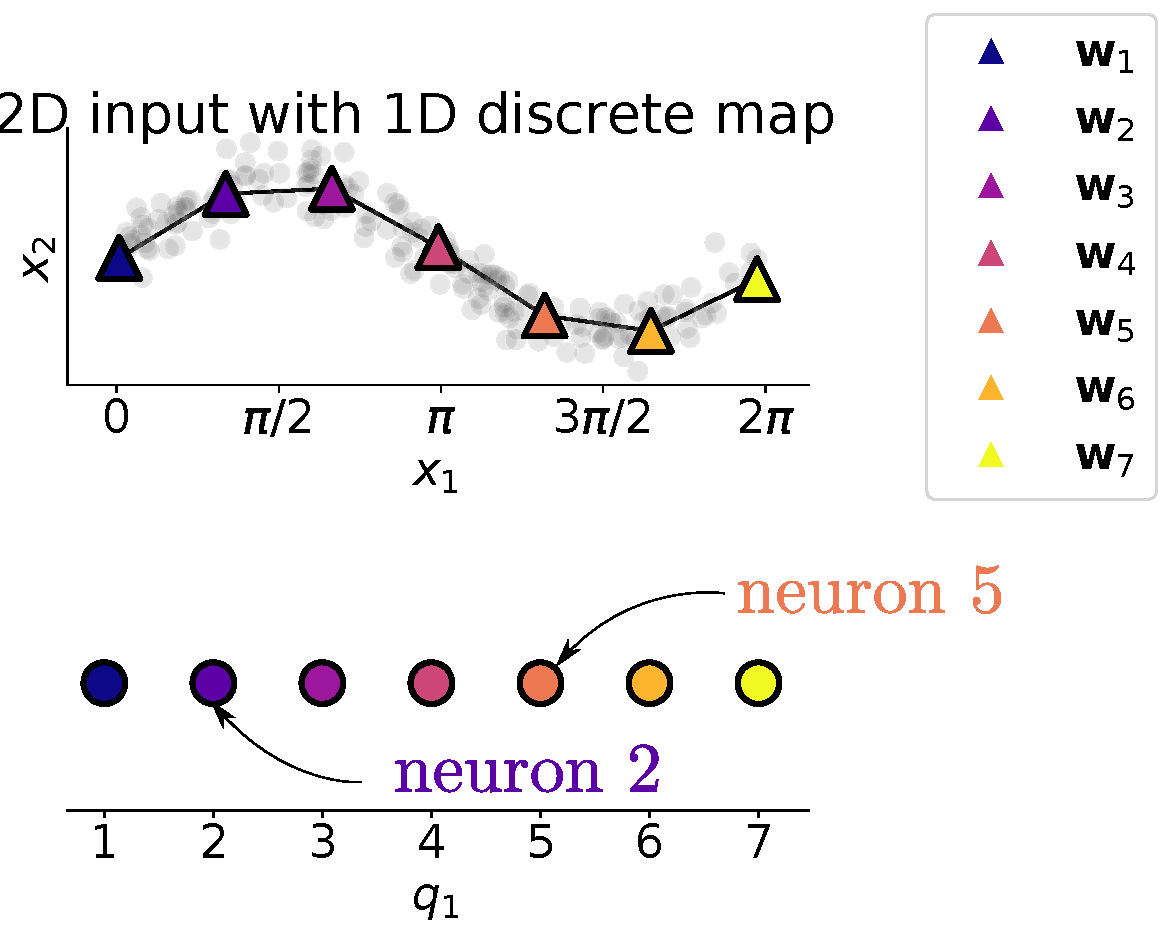
\includegraphics[width=0.5\textwidth]{img/sin_manifold_map_annot}
	\notesonly{\captionof{figure}{The 1D SOM model}}
\end{center}
}
\only<3>{
\begin{center}
\begin{minipage}{0.29\textwidth}
	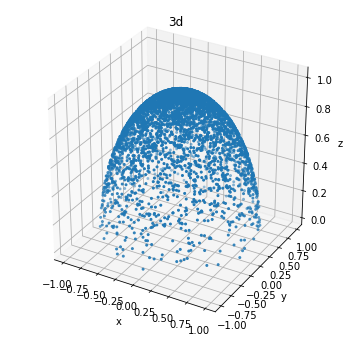
\includegraphics[width=0.9\textwidth]{img/3-a}
	\notesonly{\captionof{figure}{Bowl-shaped data in 3 dimensions}}
\end{minipage}
\begin{minipage}{0.29\textwidth}
	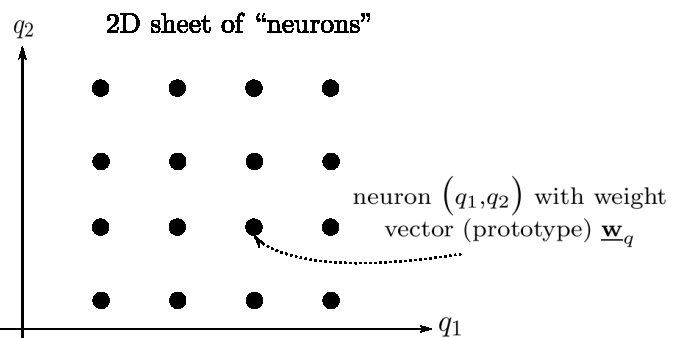
\includegraphics[width=0.99\textwidth]{img/section4_fig8}
	\notesonly{\captionof{figure}{a 2D map of neurons}}
\end{minipage}
\begin{minipage}{0.29\textwidth}
	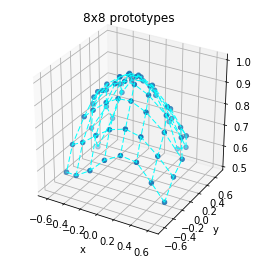
\includegraphics[width=0.9\textwidth]{img/3-b}
	\notesonly{\captionof{figure}{Prototypes fitted to the data.}}
\end{minipage}
\end{center}
}

\begin{itemize}
\only<1>{
\item The neurons form a map in a lower dimensional space.
\item The map space is discrete with coordinates $\vec q$ to describe the position of every neuron in the map (lattice)
\item Each neuron is associated with a prototype $\vec w_{\vec q}$ that lives in $N$-dim input space.
}
\only<2>{
\item In the case of a 1D map:
\begin{itemize}
\item The neurons form a chain in map space.
\item Each neuron is associated with single coordinate $q_1$ to describe its position in the chain.
\item The dimensionality of a neuron's prototype $\vec w_{q_1}$ lives in $N$-dim space (i.e. that of the input)
\end{itemize}
}
\only<3->{
\item In the case of a 2D map:
\begin{itemize}
\item The neurons form a grid (lattice) in map space.
\item Each neuron is associated with coordinates $\vec q = (q_1, q_2)^\top$ to describe its position in the grid.
\item The dimensionality of a neuron's prototype $\vec w_{\vec q}$ lives in $N$-dim space (i.e. that of the input)
\end{itemize}
}
\end{itemize}

\end{frame}

\begin{frame}%{\subsecname}

\question{What is the role of the coordinates $\vec q$ of a neuron?}

\pause

\begin{itemize}
\item It describes the neuron's position in the map. It gives us access to the neighbors of this neuron in the map.
\item This enables organizing the neurons such that the response of two neighboring neurons is more similar than that of two neurons that are far away from one another (cooperation)
\end{itemize}

\end{frame}

\begin{frame}%{\subsecname}

\question{What is the role of the prototypes $\vec w_{\vec q}$ of a neuron?}

\pause

\begin{itemize}
\item It connects the neuron to the data.
\item Enables the assignment of a sample $\vec x^{(\alpha)}$ with $\vec x \in \R^N$ and $\alpha = 1,\ldots,p$ to a neuron.\\
This is essentially clustering, but now with the possibility of a multidimensional cluster $\vec q$: \\
\begin{equation}
	m_{\vec{q}}^{(\alpha)} = \left\{ \begin{array}{ll}
		1, & \text{if } \vec q = \underset{\vec r}{\argmin} \big| \vec{x}^{(\alpha)}
			-\vec{w}_{\vec r} \big| \\\\
		0, & \text{otherwise}
	\end{array} \right.
\end{equation}
The clustering aspect can be viewed as a \emph{competition} between the neurons.
\item All prototypes collectively provide an explanation for the data. i.e. ``a 2D sheet or 1D chain that covers the space in $N$-dim space that is occupied by the data''
\end{itemize}

\end{frame}

%\subsection{Comparing SOM to clustering}

%\begin{frame}{\subsecname}

%\begin{itemize}
%\item In common:
%\begin{itemize}
%\item Protoypes live in space of the input
%\end{itemize}
%\item Differences:
%\begin{itemize}
%\item 
%\end{itemize}
%\end{itemize}

%\end{frame}
